\documentclass[a4paper, 12pt]{article}\usepackage[]{graphicx}\usepackage[]{color}
%% maxwidth is the original width if it is less than linewidth
%% otherwise use linewidth (to make sure the graphics do not exceed the margin)
\makeatletter
\def\maxwidth{ %
  \ifdim\Gin@nat@width>\linewidth
    \linewidth
  \else
    \Gin@nat@width
  \fi
}
\makeatother

\definecolor{fgcolor}{rgb}{0.345, 0.345, 0.345}
\newcommand{\hlnum}[1]{\textcolor[rgb]{0.686,0.059,0.569}{#1}}%
\newcommand{\hlstr}[1]{\textcolor[rgb]{0.192,0.494,0.8}{#1}}%
\newcommand{\hlcom}[1]{\textcolor[rgb]{0.678,0.584,0.686}{\textit{#1}}}%
\newcommand{\hlopt}[1]{\textcolor[rgb]{0,0,0}{#1}}%
\newcommand{\hlstd}[1]{\textcolor[rgb]{0.345,0.345,0.345}{#1}}%
\newcommand{\hlkwa}[1]{\textcolor[rgb]{0.161,0.373,0.58}{\textbf{#1}}}%
\newcommand{\hlkwb}[1]{\textcolor[rgb]{0.69,0.353,0.396}{#1}}%
\newcommand{\hlkwc}[1]{\textcolor[rgb]{0.333,0.667,0.333}{#1}}%
\newcommand{\hlkwd}[1]{\textcolor[rgb]{0.737,0.353,0.396}{\textbf{#1}}}%
\let\hlipl\hlkwb

\usepackage{framed}
\makeatletter
\newenvironment{kframe}{%
 \def\at@end@of@kframe{}%
 \ifinner\ifhmode%
  \def\at@end@of@kframe{\end{minipage}}%
  \begin{minipage}{\columnwidth}%
 \fi\fi%
 \def\FrameCommand##1{\hskip\@totalleftmargin \hskip-\fboxsep
 \colorbox{shadecolor}{##1}\hskip-\fboxsep
     % There is no \\@totalrightmargin, so:
     \hskip-\linewidth \hskip-\@totalleftmargin \hskip\columnwidth}%
 \MakeFramed {\advance\hsize-\width
   \@totalleftmargin\z@ \linewidth\hsize
   \@setminipage}}%
 {\par\unskip\endMakeFramed%
 \at@end@of@kframe}
\makeatother

\definecolor{shadecolor}{rgb}{.97, .97, .97}
\definecolor{messagecolor}{rgb}{0, 0, 0}
\definecolor{warningcolor}{rgb}{1, 0, 1}
\definecolor{errorcolor}{rgb}{1, 0, 0}
\newenvironment{knitrout}{}{} % an empty environment to be redefined in TeX

\usepackage{alltt}

%-----------------------------------------------------------------------------%
%	NECESSARI
%-----------------------------------------------------------------------------%
\usepackage[T1]{fontenc}
\usepackage[utf8]{inputenc} % [utf8] funziona in linux, [latin1] in windows
\usepackage[italian]{babel}
%\usepackage{lmodern}
\usepackage{txfonts}

%-----------------------------------------------------------------------------%
% FONDAMENTALE PER LA CORRETTA CREAZIONE DEI .PDF
%-----------------------------------------------------------------------------%
\usepackage{hyperref} % riferimenti incrociati e link attivi nel PDF

%-----------------------------------------------------------------------------%
% GESTIONE DEL LAYOUT
%-----------------------------------------------------------------------------%
\frenchspacing
\usepackage{microtype}
%\usepackage{layaureo}
\usepackage[margin=2cm]{geometry}

%-----------------------------------------------------------------------------%
% GESTIONE DEI TITOLI DI TAVOLE E FIGURE
%-----------------------------------------------------------------------------%
\usepackage{caption}
%\usepackage[tablename=Tavola]{caption} % con tex studio
\captionsetup[figure]{format=plain, labelfont=bf, labelsep=period, indention=0cm, justification=centering}
\captionsetup[table]{format=plain, labelfont=bf, labelsep=period, indention=0cm, justification=centering}

%-----------------------------------------------------------------------------%
% ELEMENTI GRAFICI
%-----------------------------------------------------------------------------%
\usepackage{graphicx}
\usepackage[usenames]{xcolor} % usenames abilita i 68 dvips namedcolors
\usepackage{verbatim}
\usepackage{fancyvrb} % per l'utilizzo del verbatim anche nelle note
%\usepackage{showframe} % abilita la vista dei margini
\usepackage{lipsum}
\usepackage{enumitem}

%-----------------------------------------------------------------------------%
% GESTIONE DELLE FIGURE
%-----------------------------------------------------------------------------%
\usepackage[position=bottom]{subfig}  % preferire a subfigure/subcaption

%-----------------------------------------------------------------------------%
% GESTIONE DELLE TAVOLE
%-----------------------------------------------------------------------------%
\usepackage{tabularx,booktabs}
\usepackage{multirow}
\usepackage{array}
\usepackage{lscape}


%-----------------------------------------------------------------------------%
% COMANDI FONDAMENTALI PER TABULARX
%-----------------------------------------------------------------------------%
\newcolumntype{H}{>{\centering\arraybackslash}X}
\newcolumntype{L}{>{\raggedright\arraybackslash}X}
\newcolumntype{R}{>{\raggedleft\arraybackslash}X}

\newcolumntype{2}{>{\centering\setlength{\hsize}{2\hsize}\addtolength{\hsize}{2\tabcolsep}}X}
\newcolumntype{3}{>{\centering\setlength{\hsize}{3\hsize}\addtolength{\hsize}{4\tabcolsep}}X}
\newcolumntype{4}{>{\centering\setlength{\hsize}{4\hsize}\addtolength{\hsize}{6\tabcolsep}}X}
\newcolumntype{5}{>{\centering\setlength{\hsize}{5\hsize}\addtolength{\hsize}{8\tabcolsep}}X}
\newcolumntype{6}{>{\centering\setlength{\hsize}{6\hsize}\addtolength{\hsize}{10\tabcolsep}}X}
\newcolumntype{7}{>{\centering\setlength{\hsize}{7\hsize}\addtolength{\hsize}{12\tabcolsep}}X}
\newcolumntype{8}{>{\centering\setlength{\hsize}{8\hsize}\addtolength{\hsize}{14\tabcolsep}}X}
\newcolumntype{9}{>{\centering\setlength{\hsize}{9\hsize}\addtolength{\hsize}{16\tabcolsep}}X}

%-----------------------------------------------------------------------------%
% DEFINIZIONE DI COLORI PERSONALIZZATI
%-----------------------------------------------------------------------------%
\definecolor{blu_bi}{RGB}{0,51,102}

%-----------------------------------------------------------------------------%
% DEFINIZIONE DEL FONTO PER GLI AMBIENTI TABLE E FIGURE
%-----------------------------------------------------------------------------%
\makeatletter %% Le tavole vanno in Arial
\renewenvironment{table}%
{\renewcommand\familydefault\sfdefault
	\@float{table}}
{\end@float}
\makeatother


\makeatletter %% Le figure vanno in Arial
\renewenvironment{figure}%
{\renewcommand\familydefault\sfdefault
	\@float{figure}}
{\end@float}
\makeatother


\makeatletter %% Serve solo per formattare meglio l'ambiente verbatim
\def\@xobeysp{\mbox{}\space}
\def\verbatim@font{\scriptsize\ttfamily\raggedright}
\makeatother
\IfFileExists{upquote.sty}{\usepackage{upquote}}{}
\begin{document}
%\SweaveOpts{concordance=TRUE}
\VerbatimFootnotes % per l'utilizzo del verbatim anche nelle note







%-----------------------------------------------------------------------------%
% Le tavole
%-----------------------------------------------------------------------------%
\section{Le tavole} 
\label{sec:tavole}

La tavola \ref{tab:dieci_colonne} contiene tutti gli elementi che vengono utilizzati in una tipica tavola: titolo e sottotitolo, intestazioni di colonna su più righe e più colonne, righe vuote all'interno della tavola, fonte e note sotto la tavola.

\begin{table}[h!]
  \begin{centering}
  \caption{\textbf{Dieci colonne} \protect \\ (\emph{sottotitolo})} 
  \label{tab:dieci_colonne}
% latex table generated in R 3.3.3 by xtable 1.8-2 package
% Sat Aug 18 20:54:01 2018
\begingroup\fontsize{7pt}{8pt}\selectfont
\begin{tabularx}{\textwidth}{LLLHHHRRRR}
   
\toprule
% riga 1
  \multicolumn{10}{>{\centering\setlength{\hsize}{9\hsize}\addtolength{\hsize}{16\tabcolsep}}X}{Unione di dieci colonne} \\
  \cmidrule(lr){1-10}
% riga 2
  Periodo & \multicolumn{9}{9}{\lipsum[1]} \\ 
  \cmidrule(lr){2-10}
% riga 3
  & & & \multicolumn{7}{7}{\lipsum[1]} \\
  \cmidrule(lr){3-3} \cmidrule(lr){4-10}
% riga 4
  & &  \multirow{2}{\linewidth}{\centering \emph{di cui: } sofferenze} & & 
  \multirow{2}{\linewidth}{\centering Assicu- razioni, fondi pensione e altre istituzioni finanziarie} & 
  \multirow{2}{\linewidth}{\centering Societa non finanziarie} & 
  \multicolumn{4}{4}{Famiglie} \\
  \cmidrule(lr){7-10}
% riga 5  
  & & & & & & & 
  \multicolumn{1}{H}{Credito al consumo} & \multicolumn{1}{H}{Acquisto di abitazioni \vspace{1cm}} & \multicolumn{1}{H}{Altri prestiti} \\
\midrule
 Italia & 2 & 3 & 4 & 5 & 6 & 7 & 8 & 9 & 10 \\10,1 & 11 & 12,1 & 13,1 & 14,1 & 15,1 & 16,1 & 17,1 & 18,1 & 19,1 \\ 
  10,2 & 11 & 12,2 & 13,2 & 14,2 & 15,2 & 16,2 & 17,2 & 18,2 & 19,2 \\ 
  10,3 & 11 & 12,3 & 13,3 & 14,3 & 15,3 & 16,3 & 17,3 & 18,3 & 19,3 \\ 
  10,4 & 11 & 12,4 & 13,4 & 14,4 & 15,4 & 16,4 & 17,4 & 18,4 & 19,4 \\ 
  10,5 & 12 & 12,5 & 13,5 & 14,5 & 15,5 & 16,5 & 17,5 & 18,5 & 19,5 \\ 
   Francia & & & & & & & & & \\10,6 & 12 & 12,6 & 13,6 & 14,6 & 15,6 & 16,6 & 17,6 & 18,6 & 19,6 \\ 
  10,7 & 12 & 12,7 & 13,7 & 14,7 & 15,7 & 16,7 & 17,7 & 18,7 & 19,7 \\ 
  10,8 & 12 & 12,8 & 13,8 & 14,8 & 15,8 & 16,8 & 17,8 & 18,8 & 19,8 \\ 
  10,9 & 12 & 12,9 & 13,9 & 14,9 & 15,9 & 16,9 & 17,9 & 18,9 & 19,9 \\ 
  11,0 & 12 & 13,0 & 14,0 & 15,0 & 16,0 & 17,0 & 18,0 & 19,0 & 20,0 \\ 
   \bottomrule\end{tabularx}
\endgroup

  \end{centering}
  {\scriptsize 
    Fonte: \lipsum[1]
    (1) \verb|align="cLHHHHHHHHH"|. Il primo valore non viene considerato perché si riferisce a rownames.\\
    (2) \verb|digits=c(0,1,0,1,1,1,1,1,1,1,1)|. Il primo valore non viene considerato perché si riferisce a rownames.\\
    (3) Per aggiungere spazio sotto la tavola inserire il comando \verb|\\[5\baselineskip]|.
  }
  \\[1\baselineskip]
\end{table}

%-----------------------------------------------------------------------------%

\subsection{Il font (family e size)} 
\label{sec:font}
Il font per le tavole è l'Arial, caricato con il pacchetto txfonts (\verb|\usepackage{txfonts}|) e settato per le tavole con un \verb|\renewenvironment{table}| all'interno del preambolo:
\begin{verbatim}
\makeatletter %% Le tavole vanno in Arial
\renewenvironment{table}%
{\renewcommand\familydefault\sfdefault
	\@float{table}}
{\end@float}
\makeatother
\end{verbatim}

Il fontsize e l'interlinea della tavola sono definiti nella funzione \verb|print()| del file .R impostando l'argomento \verb|size="\\fontsize{7pt}{8pt}\\selectfont"|, rispettivamente fontsize e linespace.

\subsection{Il titolo (e il sottotitolo)} 
\label{sec:titolo}

%-----------------------------------------------------------------------------%

Il titolo (e il relativo sottotitolo) e il label della tavola possono essere definiti o nel file .R, nella funzione \verb|xtable()|, o direttamente nel file .Rnw. Nel primo caso l'ambiente table (\verb|\begin{table} \end{table}|) è creato dalla funzione \verb|print()| nel file .R, impostando l'argomento \verb|floating=TRUE|; nel secondo caso l'ambiente table deve essere creato manualmente all'interno del file .Rnw impostando l'argomento \verb|floating=FALSE|. Il secondo metodo è sicuramente più flessibile in quanto offre la possibilità di gestire meglio gli altri elementi della tavola, come la fonte e le note.

\begin{verbatim}
# Metodo 1: floating=T
carb0100 <- xtable(
  a10,
  caption=c('Dieci colonne'),
  label=c('tab:dieci_colonne'),
  align = "cLHHHHHHHHH", # inserire un valore in piu' rispetto al numero delle colonne
  digits=c(0,1,0,1,1,1,1,1,1,1,1) # inserire un valore in piu' rispetto al numero delle colonne
)
print(carb0100,
  floating=T, # se TRUE crea automaticamente l'ambiente \begin{table}
  #floating=F, # se FALSE crea solo l'ambiente tabularx. L'ambiente table (con caption e label) va creato direttamente nel file .Rnw
)
\end{verbatim}


\begin{verbatim}
# Metodo 2: floating=F
carb0100 <- xtable(
  a10,
  #caption=c('Dieci colonne'),
  #label=c('tab:dieci_colonne'),
  align = "cLHHHHHHHHH", # inserire un valore in piu' rispetto al numero delle colonne.
  digits=c(0,1,0,1,1,1,1,1,1,1,1) # inserire un valore in piu' rispetto al numero delle.
)
print(carb0100,
  #floating=T, # se TRUE crea automaticamente l'ambiente \begin{table}
  floating=F, # se FALSE crea solo l'ambiente tabularx. L'ambiente table (con caption e label) va creato direttamente nel file .Rnw
)
\end{verbatim}

Gli elementi del blocco del titolo (allineamento, separatore, grassetto, ecc.) sono definiti e gestiti dal comando \verb|\captionsetup[table]{}| del pacchetto \verb|caption|: 
\begin{verbatim} \captionsetup[table]{format=plain, labelfont=bf, labelsep=period, indention=0cm, justification=centering}\end{verbatim}.

Per forzare un invio a capo all'interno del titolo (\verb|\caption|) è necessario anteporre il comando \verb|\protect| al simbolo dell'invio \verb|\\|:
\begin{verbatim}\caption{\textbf{Titolo} \protect \\ (\emph{sottotitolo})} \end{verbatim}. 

%-----------------------------------------------------------------------------%

\subsection{Le intestazioni di colonna} 
\label{sec:intestazioni}
Le intestazioni di colonna sono allineate al centro; eventuali unioni di celle sono realizzate con i comandi \verb|\multirow{n}{lunghezza}{testo}| e  \verb|\multicolumn{n}{>{lunghezza}X}{testo}| per gestire gli invii a capo mantenendo contemporaneamente l'allineamento centrato. La lunghezza esatta di una \verb|multicolumn{n}| è data dalla formula $n \cdot hsize + [(n \cdot 2)-2] \cdot tabcolsep$
\footnote{La lunghezza della colonna unita calcolata automaticamente da \verb|tabularx| è più piccola rispetto alla somma delle lunghezze delle colonne originarie: infatti, poiché l'ambiente \verb|\tabularx| crea un \emph{padding} (chiamato \verb|\tabcolsep|) a sinistra e a destra di ogni colonna, quando le colonne vengono unite la lunghezza della nuova colonna perde la somma di tutti i \verb|\tabcolsep|, cioè due (uno a sinistra, uno a destra) per ogni colonna originaria. In una unione di tre colonne lunghe $2cm$ ciascuna, la colonna unita risultante non sarà lunga $6cm$, ma $6cm-(3 \cdot 2 \cdot tabcolsep)$. Di conseguenza per avere una \verb|multicolumn{n}| che si allunghi per tutto lo spazio disponibile bisogna settare una lunghezza (\verb|\setlength{\hsize}|) pari a $n$ (\verb|{n\hsize}|) e aggiungere a questa lunghezza (\verb|\addtolength{\hsize}|) i \verb|\tabcolsep| che si sono persi nell'unione effettuata da \verb|tabularx|; in particolare bisogna aggiungerne due per ogni colonna unita meno uno a sinistra e uno a destra: $(2 \cdot n)-2$. Ad esempio, la lunghezza corretta di una \verb|\multicolumn{9}| di 9 colonne è: $9 \cdot hsize + [(2 \cdot 9)-2] \cdot tabcolsep \Rightarrow 9 \cdot hsize + 16 \cdot tabcolsep$ dove 9 è il numero delle colonne e 16 è il numero dei padding che vanno ri-aggiunti (2 per ognuna delle nove colonne meno uno a destra e uno a sinistra della colonna unita).}.

\begin{verbatim}
\\multirow{2}{\\linewidth}{\\centering Testo}
\\multirow{3}{\\linewidth}{\\centering Testo}
\\multirow{4}{\\linewidth}{\\centering Testo}
\\multicolumn{2}{>{\\centering\\setlength{\\hsize}{2\\hsize}\\addtolength{\\hsize}{2\\tabcolsep}}X}{\\lipsum[1]}
\\multicolumn{3}{>{\\centering\\setlength{\\hsize}{3\\hsize}\\addtolength{\\hsize}{4\\tabcolsep}}X}{\\lipsum[1]}
\\multicolumn{4}{>{\\centering\\setlength{\\hsize}{4\\hsize}\\addtolength{\\hsize}{6\\tabcolsep}}X}{\\lipsum[1]}
\\multicolumn{9}{>{\\centering\\setlength{\\hsize}{9\\hsize}\\addtolength{\\hsize}{16\\tabcolsep}}X}{\\lipsum[1]}
\end{verbatim}

Per evitare di ripetere ogni volta la stringa del \verb|\multicolumn{}| è possibile creare dei \verb|\newcolumntype{nome}| nel preambolo e poi richiamarli nella tavola:

\begin{verbatim}
\documentclass[]{article}
% Preambolo
\newcolumntype{4}{>{\centering\setlength{\hsize}{4\hsize}\addtolength{\hsize}{6\tabcolsep}}X}
\begin{document}
% Inizio documento
\multicolumn{4}{4}{Famiglie}
\end{document}
\end{verbatim}


Ai fini di mantenere una corretta formattazione nelle celle singole (mantenere il testo centrato su più linee) è necessario utilizzare il comando \verb|multicolumn{n}| anche se $n=1$. 
\begin{verbatim}
\\multicolumn{1}{H}{Credito al consumo} & \\multicolumn{1}{H}{Acquisto di abitazioni \\vspace{1cm}} & \\multicolumn{1}{H}{Altri prestiti}
\end{verbatim}


Quando il contenuto di una cella è molto lungo e supera il limite verticale della cella stessa occorre aggiungere spazio verticale in una qualsiasi delle celle dell'ultima riga con il comando \verb|\\vspace{h}| (ad esempio \verb|\\vspace{1cm}|; fig. \ref{fig:vspace}).
\begin{figure}[h!]
\centering%

\caption{Utilizzo del comando vspace}%
\label{fig:vspace}%

\subfigure[{Senza spazio verticale aggiuntivo sotto la colonna \emph{Acquisto di abitazioni}.}]{\includegraphics[width=0.4\linewidth]{figure/vspace0}\label{fig:VariazioneRelativa}}\quad
\subfigure[{Con spazio verticale aggiuntivo (vspace{1cm}) sotto la colonna \emph{Acquisto di abitazioni}.}]{\includegraphics[width=0.4\linewidth]{figure/vspace1}\label{fig:VariazioneAssoluta}}

\end{figure}

%-----------------------------------------------------------------------------%

\subsection{Altro} 
\label{sec:altro}
Il comando addtorow è una lista che contiene al suo interno due elementi: una lista chiamata \emph{pos} e un vettore chiamato \emph{command}. La lista pos e il vettore command devono avere lo stesso numero di elementi: ogni elemento di pos identifica una riga della tavola (da 0 --- prima della prima riga --- a nrow --- dopo l'ultima riga ---) dove verrà posizionato il corrispettivo elemento di command.

{\scriptsize \begin{verbatim}
addtorow <- list()
addtorow$pos <- list()
addtorow$pos[[1]] <- 0
addtorow$pos[[2]] <- 0
addtorow$pos[[3]] <- 5
addtorow$pos[[4]] <- nrow(a10)

addtorow$command <- c(
  intestazione, # primo elemento di command, che va nella riga identificata dal primo elemento di pos (riga 0)
  'Italia & 2 & 3 & 4 & 5 & 6 & 7 & 8 & 9 & 10 \\\\', # secondo elemento di command che va nella riga identificata dal secondo elemento di pos (riga 0)
  'Francia & & & & & & & & & \\\\', # terzo elemento di command che va nella riga identificata dal terzo elemento di pos (riga 5)
  '\\bottomrule' # quarto elemento di command che va nella riga identificata dal quarto elemento di pos (ultima riga)
)
\end{verbatim}}


%-----------------------------------------------------------------------------%
% Le figure
%-----------------------------------------------------------------------------%

\section{Le figure} 
\label{sec:figure}



% 
% \begin{figure}[!t]
% 	\caption{Grafico di prova}%
% 	\label{fig:prova}%
% <<g3, out.width='17cm', fig.asp=0.623, fig.show='hold', echo=FALSE, warning=FALSE>>=
% ggplot(g3, aes(x=variable, fill=variable)) +
% 	geom_bar()
% @
% \end{figure}



\begin{figure}[bth]
\centering
\caption{Ambiente subfig con due subfloat}
\label{subfig}
	\subfloat[Subfloat 1]{\label{subfloat_1}
\begin{knitrout}
\definecolor{shadecolor}{rgb}{0.969, 0.969, 0.969}\color{fgcolor}
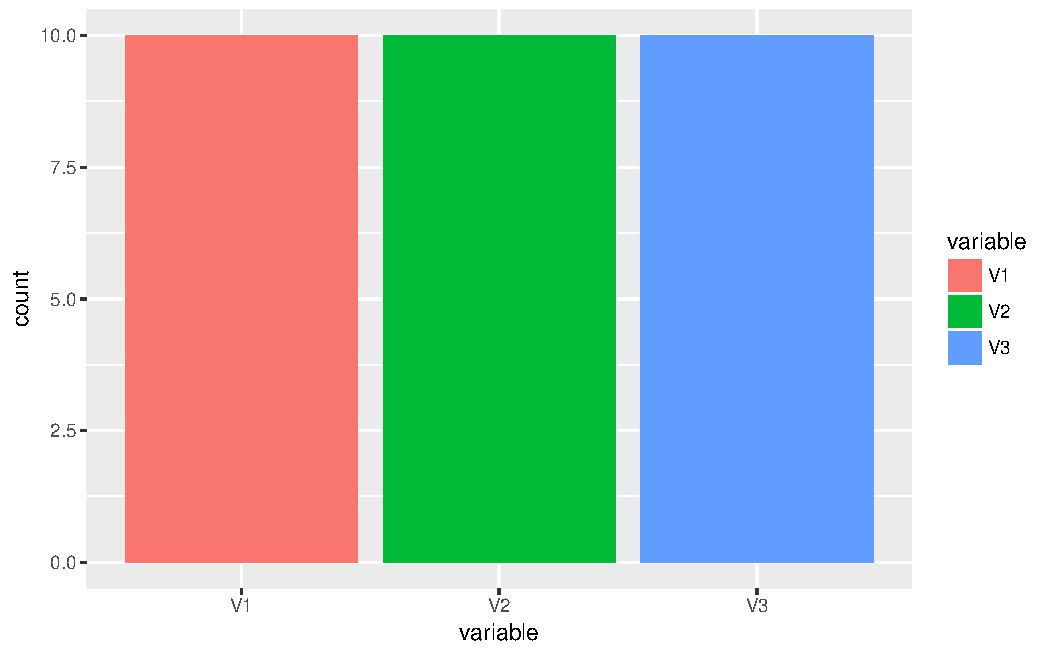
\includegraphics[width=.45\textwidth]{figure/g3-1} 

\end{knitrout}
	}\qquad
	\subfloat[Subfloat 2]{\label{subfloat_2}
\begin{knitrout}
\definecolor{shadecolor}{rgb}{0.969, 0.969, 0.969}\color{fgcolor}
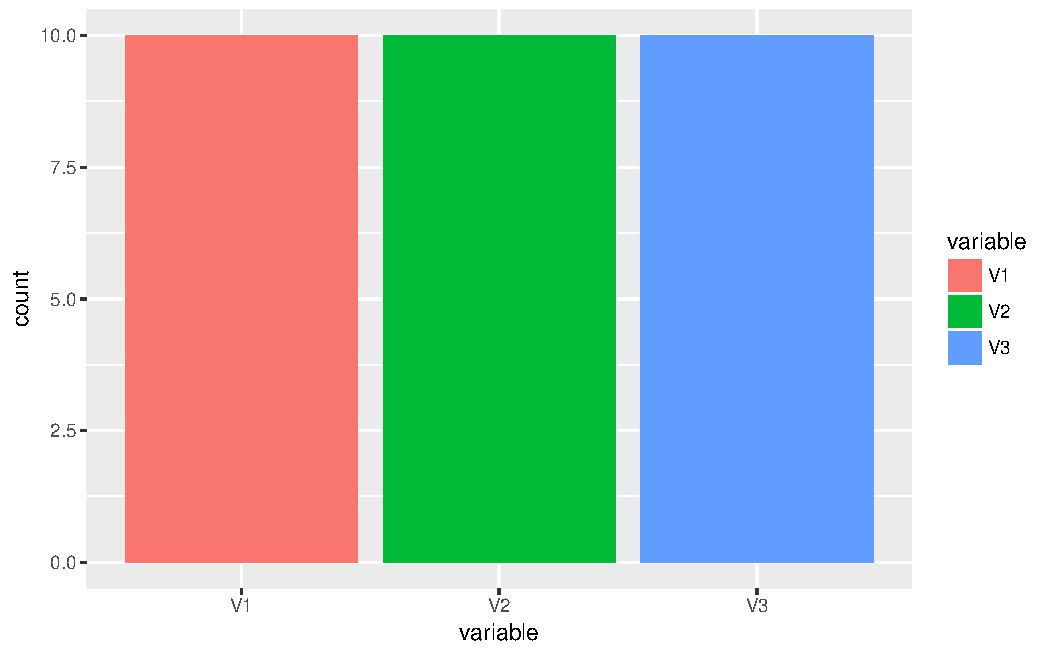
\includegraphics[width=.45\textwidth]{figure/g4-1} 

\end{knitrout}
	}
\end{figure}



\vspace*{\fill}
\newpage

\begin{center}
\includegraphics[width=0.4\linewidth]{figure/logo.png}\\[1\baselineskip]
\end{center}


\noindent\makebox[\linewidth][c]{%
  \colorbox{blu_bi}{%
    \parbox{\paperwidth}{      
        \centering \color{white} { \Huge \textbf{Comunicato stampa}\\[.2\baselineskip]
        \small{DIFFUSO A CURA DEL SERVIZIO SEGRETERIA PARTICOLARE DEL DIRETTORIO E COMUNICAZIONE}}      
    }%
  }%
}

\end{document}
